\def\focusbranch{
    Nhánh tập trung đối tượng\index{nhánh tập trung đối tượng} của RetinaFocus được xây dựng dựa trên mô hình AutoFocus \cite{najibi2019autofocus}, một mô hình giải quyết bài toán xử lý ảnh chất lượng cao rất hiệu quả.
    Ý tưởng của AutoFocus \cite{najibi2019autofocus} hướng đến việc loại bỏ những điểm ảnh\index{điểm ảnh} dư thừa mà mô hình phải xử lý trong quá trình dự đoán nhưng vẫn giữ được ý tưởng về việc sử dụng Image Pyramids.
    Ý tưởng của nhánh tập trung đối tượng\index{nhánh tập trung đối tượng} được thiết kế nhằm dự đoán những khu vực đáng chú ý ở trên ảnh và loại bỏ những khu vực khả năng cao không chứa đối tượng ở những kích thước ảnh lớn hơn, từ đó, tiết kiệm được rất nhiều chi phí tính toán trong quá trình dự đoán của mô hình.

    \noindent
    Dựa trên mô hình AutoFocus \cite{najibi2019autofocus}, nhánh tập trung đối tượng\index{nhánh tập trung đối tượng} của RetinaFocus gồm hai thành phần là \textit{Thuật toán Focus Pixel} và \textit{Thuật toán sinh Focus Chips}.
    Ngoài ra, bổ sung thêm \textit{Thuật toán Focus Stacking} vào nhánh xác định đối tượng\index{nhánh xác định đối tượng}. \\

    \noindent
    \textbf{\textit{Thuật toán Focus Pixel}} \\
    Tương tự như trong mô hình AutoFocus \cite{najibi2019autofocus}, thuật toán Focus Pixel là thuật toán giúp chúng ta có thể xác định được vị trí khu vực có khả năng chứa đối tượng và cần zoom trên ảnh.
    Ý tưởng của thuật toán Focus Pixel  dựa trên việc khi ta đưa đầu vào một ảnh có kích thước $X \times Y$ qua một khối Conv, bản đồ đặc trưng\index{bản đồ đặc trưng} mà ta thu được có kích thước $X' \times Y'$, trong đó: $X' = \lceil \frac{X}{s} \rceil$, $Y' = \lceil \frac{Y}{s} \rceil$, và $s$ là stride của cả khối Conv.
    Từ đó ta có thể ngầm hiểu rằng một điểm ảnh\index{điểm ảnh} trên bản đồ đặc trưng\index{bản đồ đặc trưng} có kích thước $X' \times Y'$ đại diện cho một khu vực có kích thước $s \times s$ trên ảnh đầu vào. \\
    Cụ thể, Focus Pixel  xác định các điểm ảnh\index{điểm ảnh} trên mask là các \textit{điểm ảnh cần được focus} nếu như điểm ảnh\index{điểm ảnh} đó có overlap với grountruth hộp giới hạn\index{hộp giới hạn} của đối tượng có kích thước nhỏ.
    Tiếp theo, các điểm ảnh\index{điểm ảnh} trên mask là các \textit{điểm ảnh không cần quan tâm} nếu như điểm ảnh\index{điểm ảnh} đó có overlap với groundtruth\index{groundtruth} hộp giới hạn\index{hộp giới hạn} của đối tượng có kích thước lớn hoặc rất nhỏ.
    Cuối cùng, các \textit{điểm ảnh không cần được focus} trên mask là các điểm ảnh\index{điểm ảnh} còn lại.

    \[l = 
        \begin{cases}
            1, & IoU\index{IoU}(GT, l) > 0, a < \sqrt{GTArea} < b \\
            -1, & IoU\index{IoU}(GT, l) > 0, \sqrt{GTArea} < a  \\
            -1, & IoU\index{IoU}(GT, l) > 0, b < \sqrt{GTArea} < c  \\
            0, & \text{otherwise}
        \end{cases}
    \]

    \noindent
    trong đó: \\
    - $IoU\index{IoU}(GT, l)$ là chỉ số IoU\index{IoU} giữa khu vực $s \times s$ và groundtruth\index{groundtruth} hộp giới hạn\index{hộp giới hạn} của đối tượng trên ảnh đầu vào. \\
    - $GTArea$ là diện tích của groundtruth\index{groundtruth} hộp giới hạn\index{hộp giới hạn} của đối tượng trên ảnh đầu vào. \\
    Nếu một khu vực $s \times s$ overlap với nhiều groundtruth\index{groundtruth} hộp giới hạn\index{hộp giới hạn} của đối tượng, thì điểm ảnh\index{điểm ảnh} đó được ưu tiên là một Focus Pixel .

    \noindent
    Trong các thí nghiệm mà nhóm tác giả của AutoFocus \cite{najibi2019autofocus} thực hiện, nhóm tác giả sử dụng các tham số $a = 5, b = 64, c = 90$ nghĩa là các groundtruth\index{groundtruth} hộp giới hạn\index{hộp giới hạn} có kích thước từ $5 \times 5$ đến $64 \times 64$ là các hộp giới hạn\index{hộp giới hạn} cần được focus, các groundtruth\index{groundtruth} hộp giới hạn\index{hộp giới hạn} có kích thước dưới $5 \times 5$ hoặc từ $64 \times 64$ đến $90 \times 90$ là các hộp giới hạn\index{hộp giới hạn} không cần quan tâm và các groundtruth\index{groundtruth} hộp giới hạn\index{hộp giới hạn} có kích thước trên $90 \times 90$ là các hộp giới hạn\index{hộp giới hạn} không cần được focus.
    
    \begin{figure}[H]
        \centering
        \subfigure[]{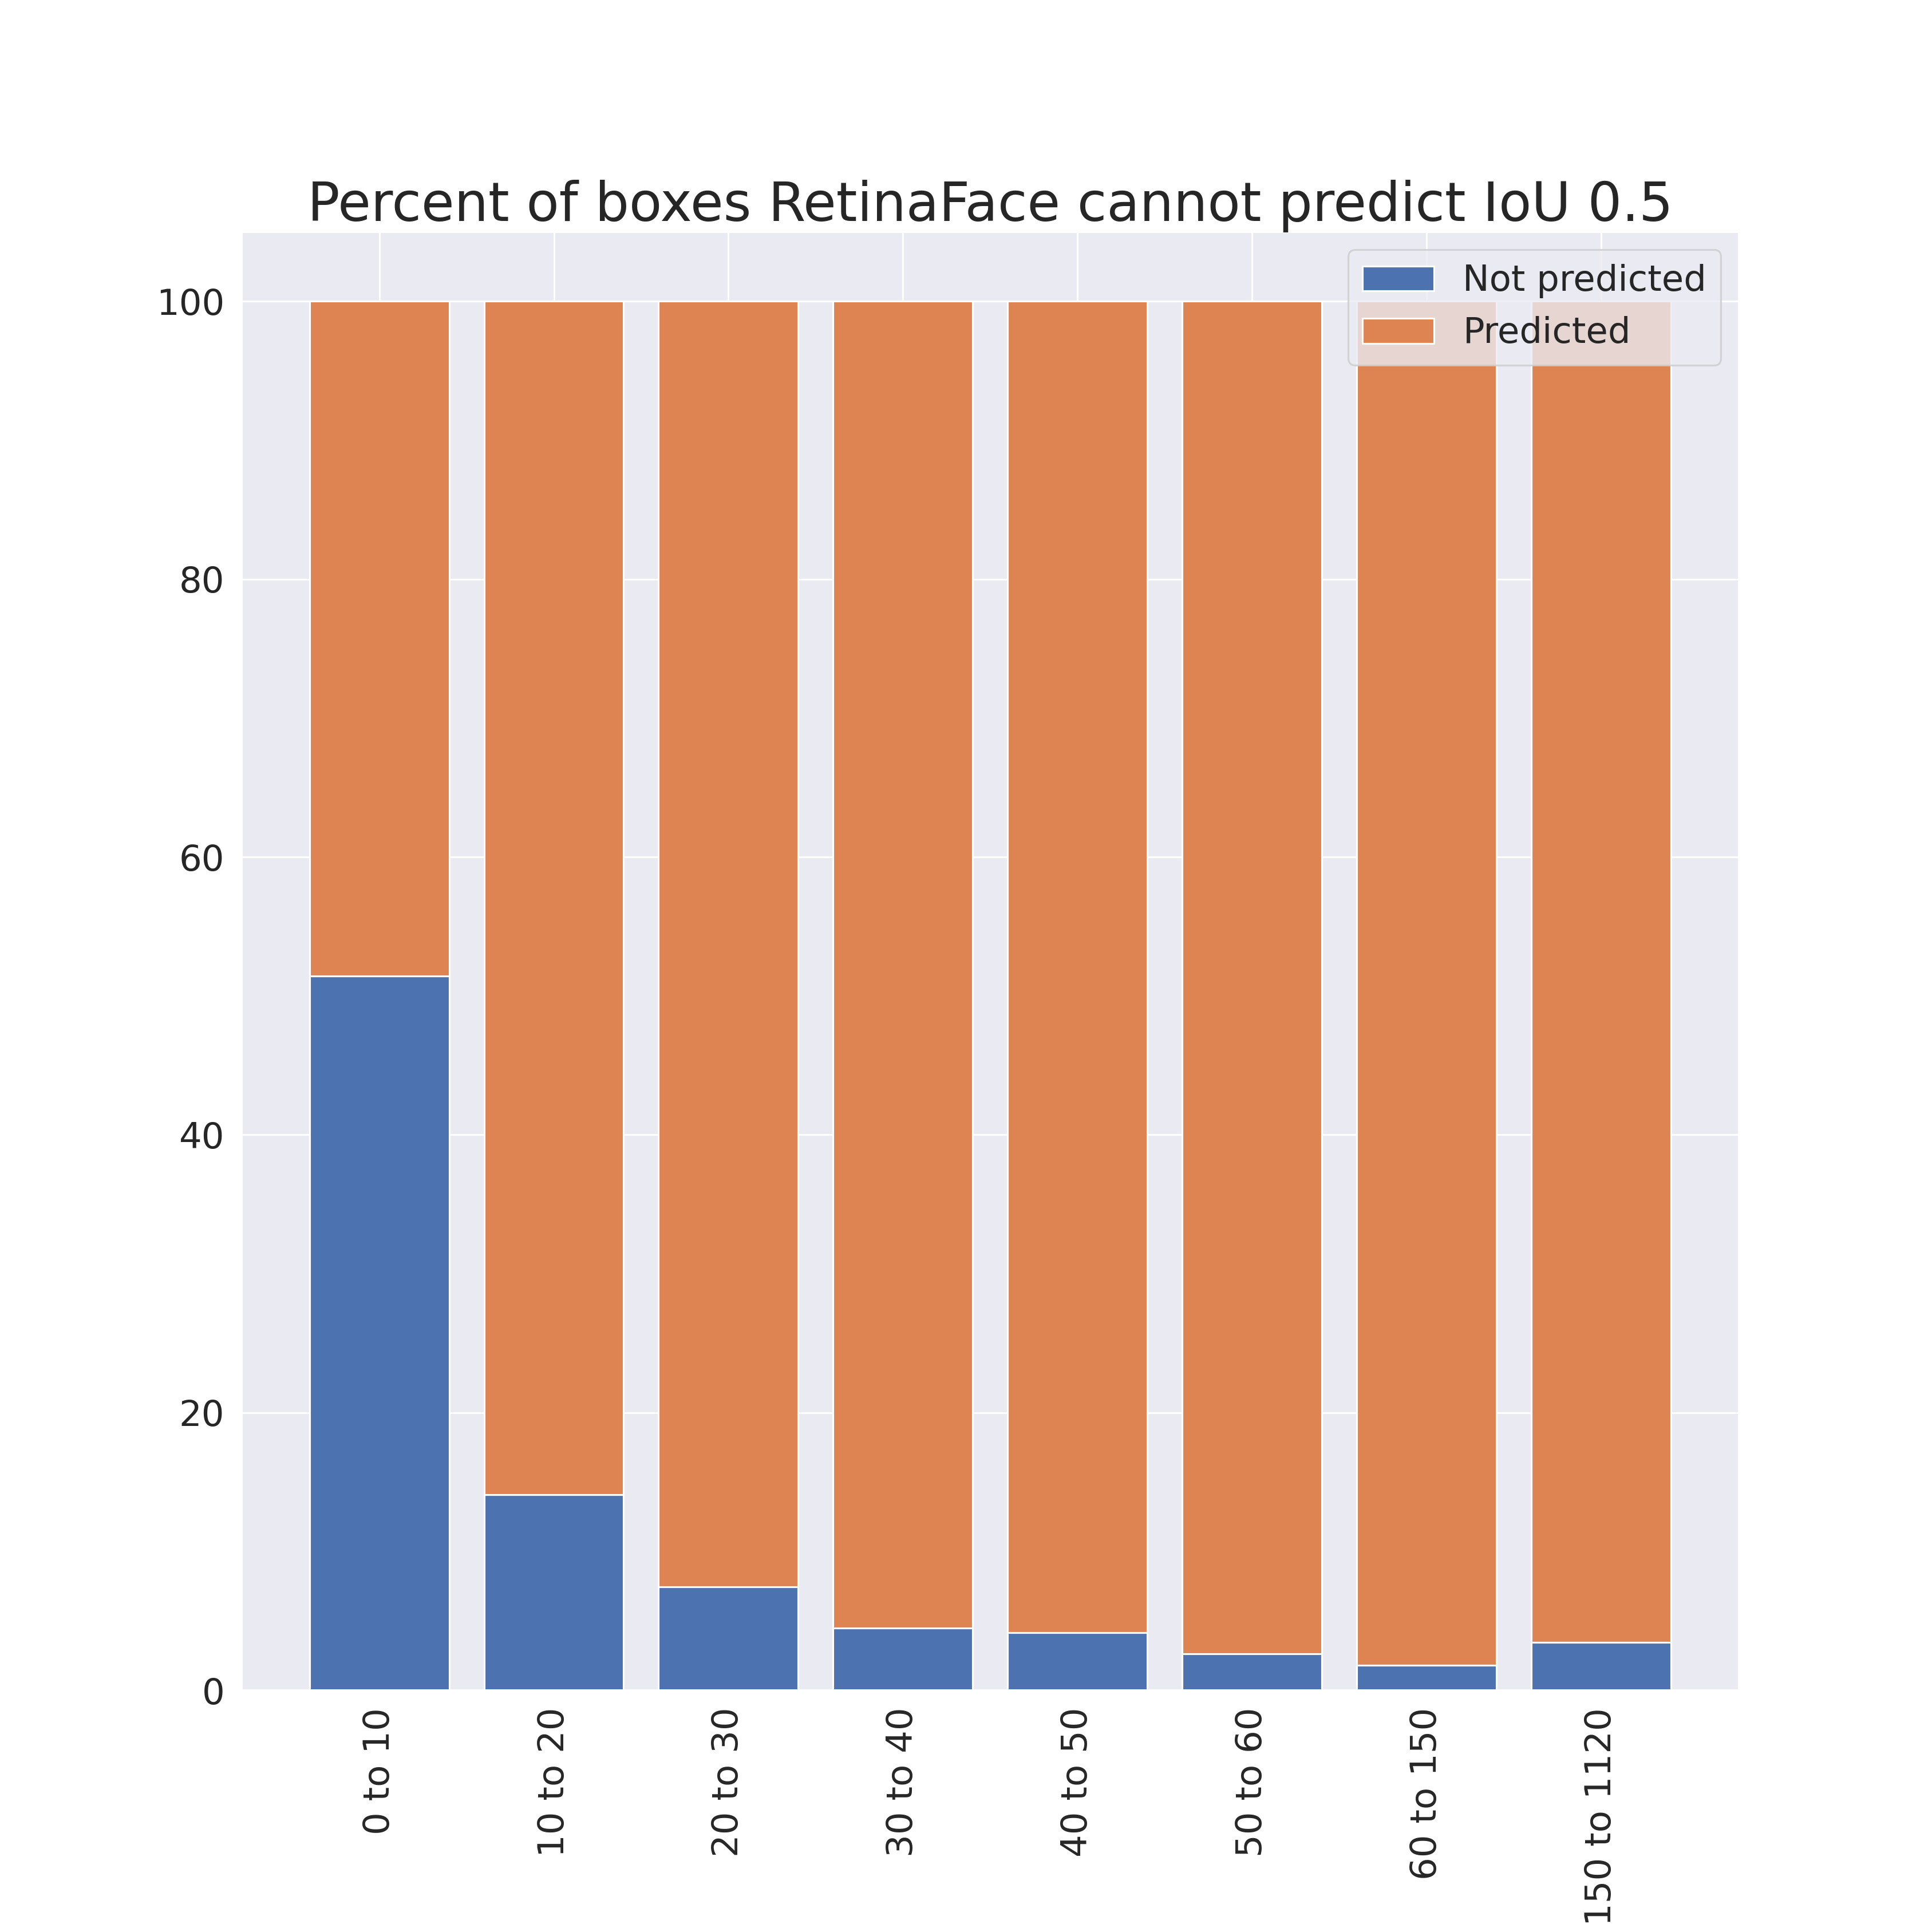
\includegraphics[width=7.3cm, trim={2.5cm 0cm 1.7cm 3.3cm}, clip]{images/retinafocus_iou_50_compare_percent}} 
        \subfigure[]{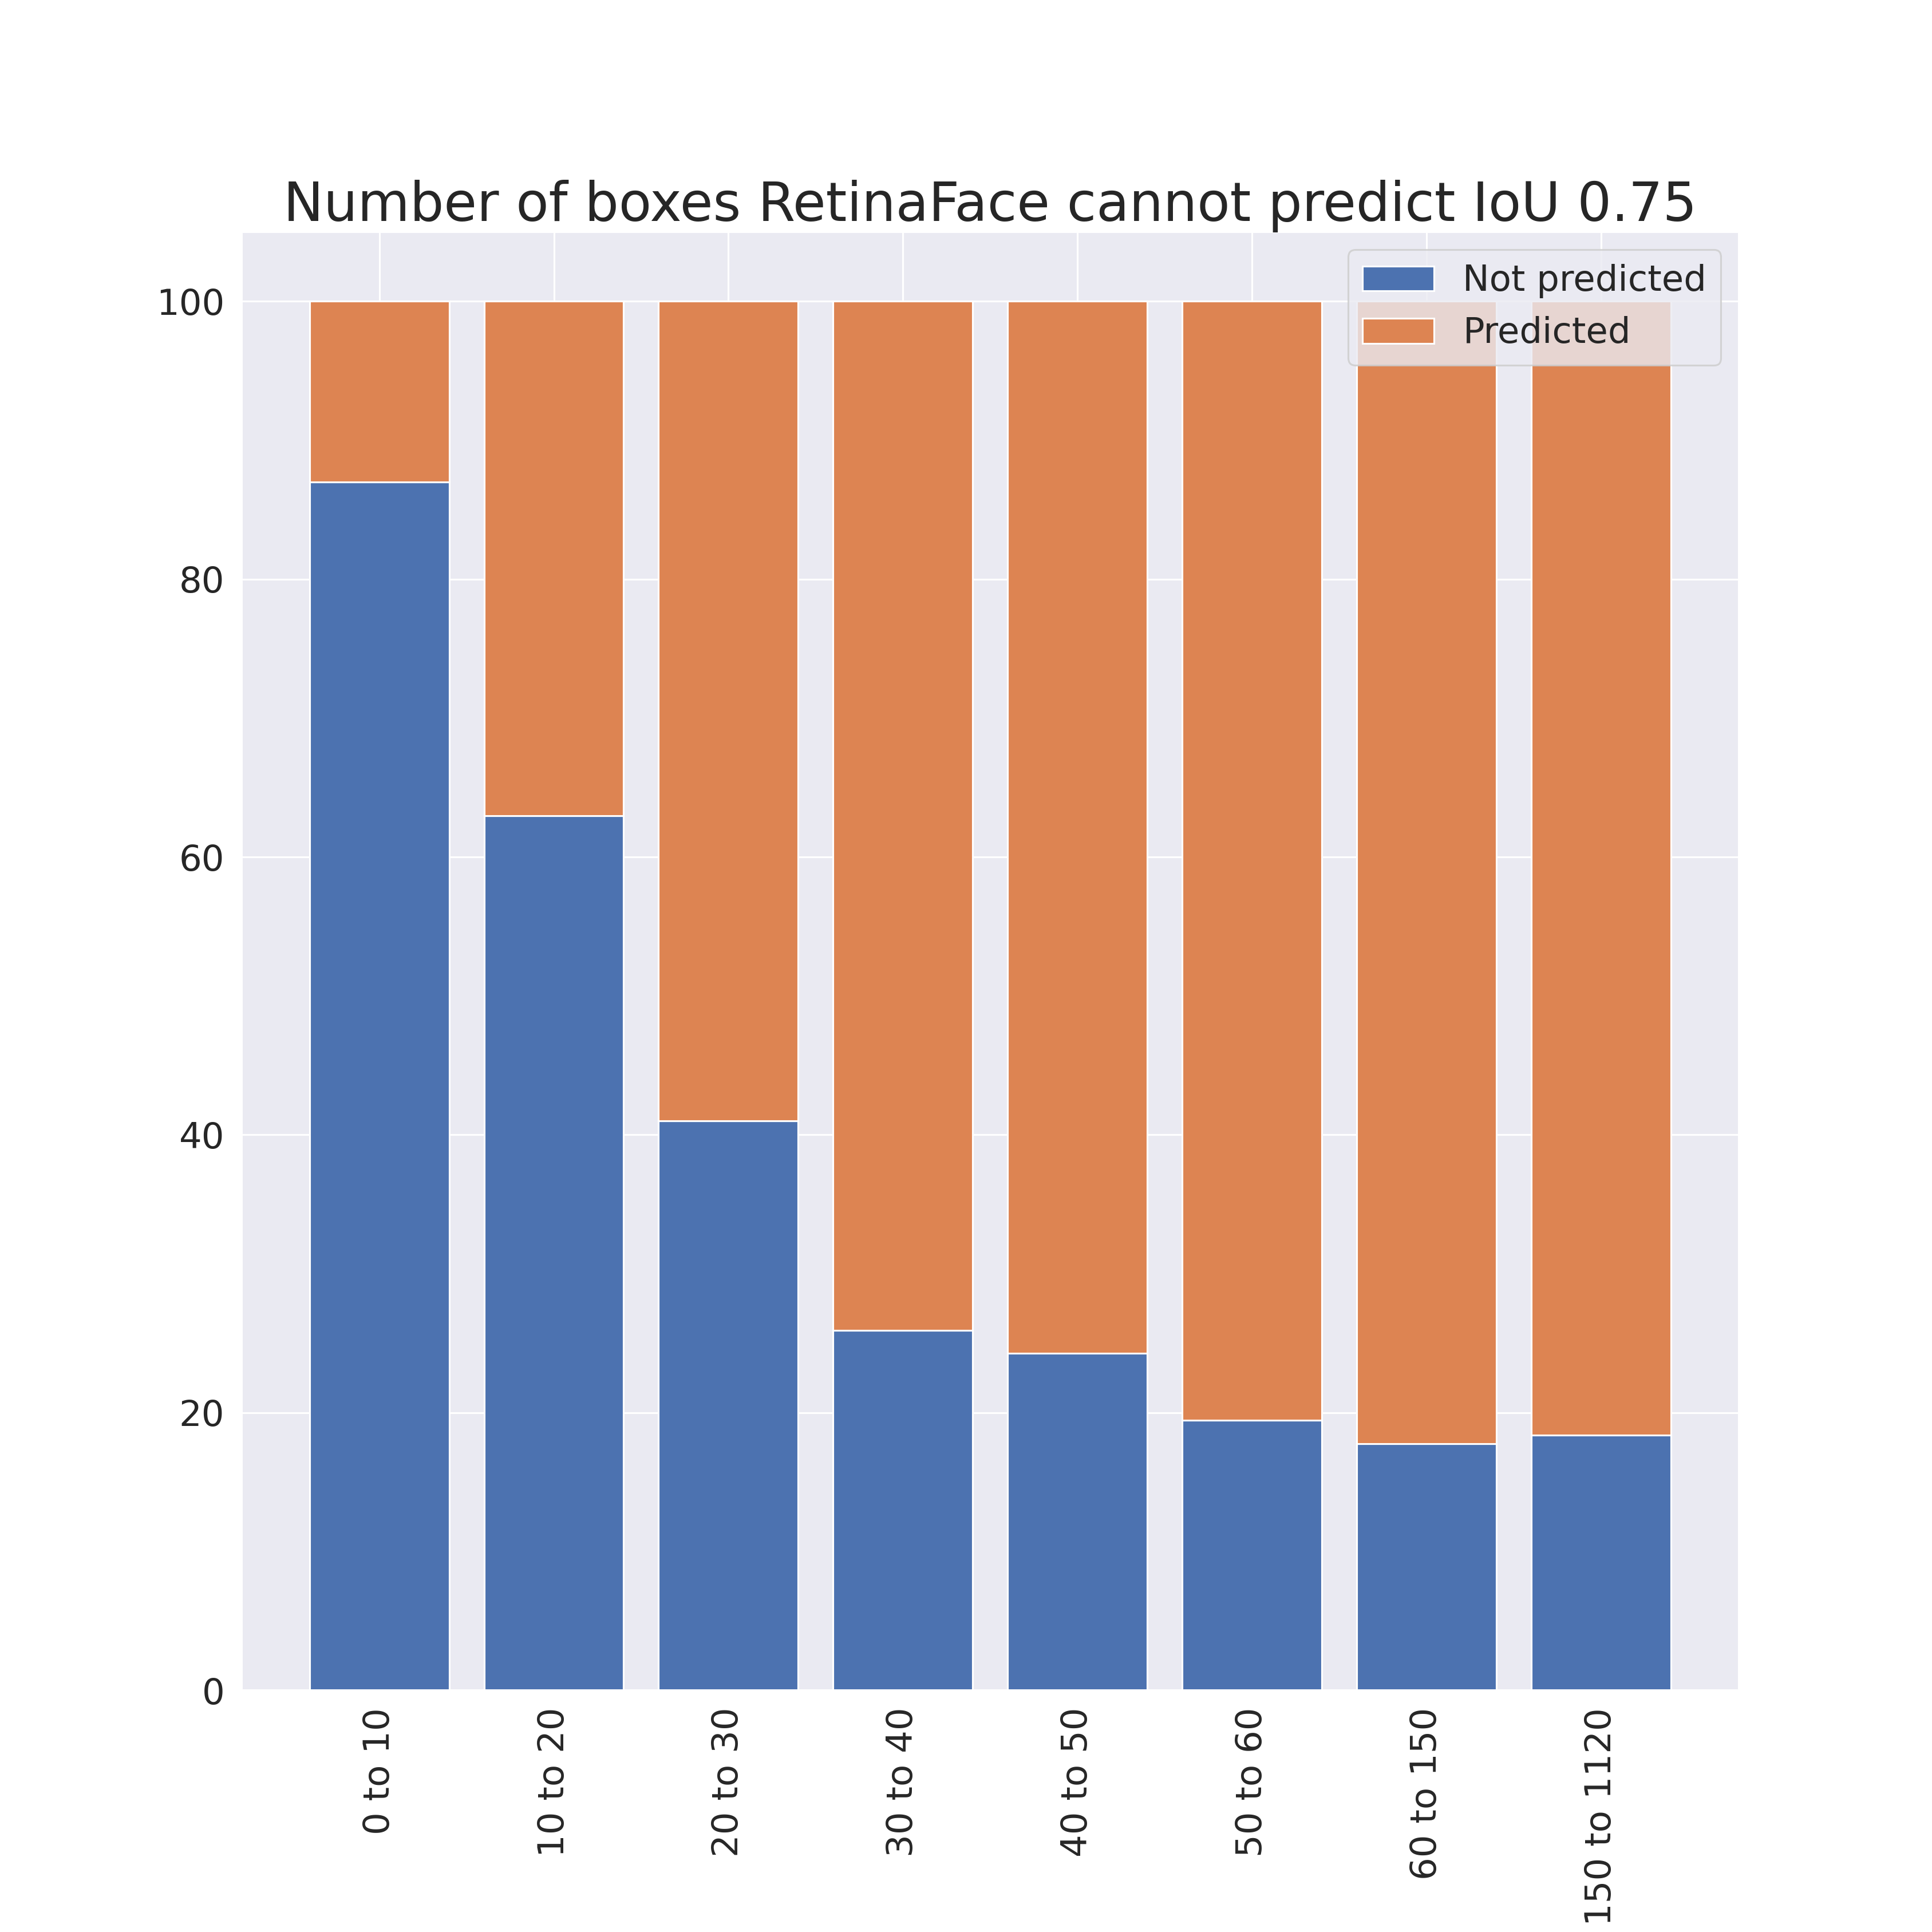
\includegraphics[width=7.3cm, trim={2.5cm 0cm 1.7cm 3.3cm}, clip]{images/retinafocus_iou_75_compare_percent}} 
        \subfigure[]{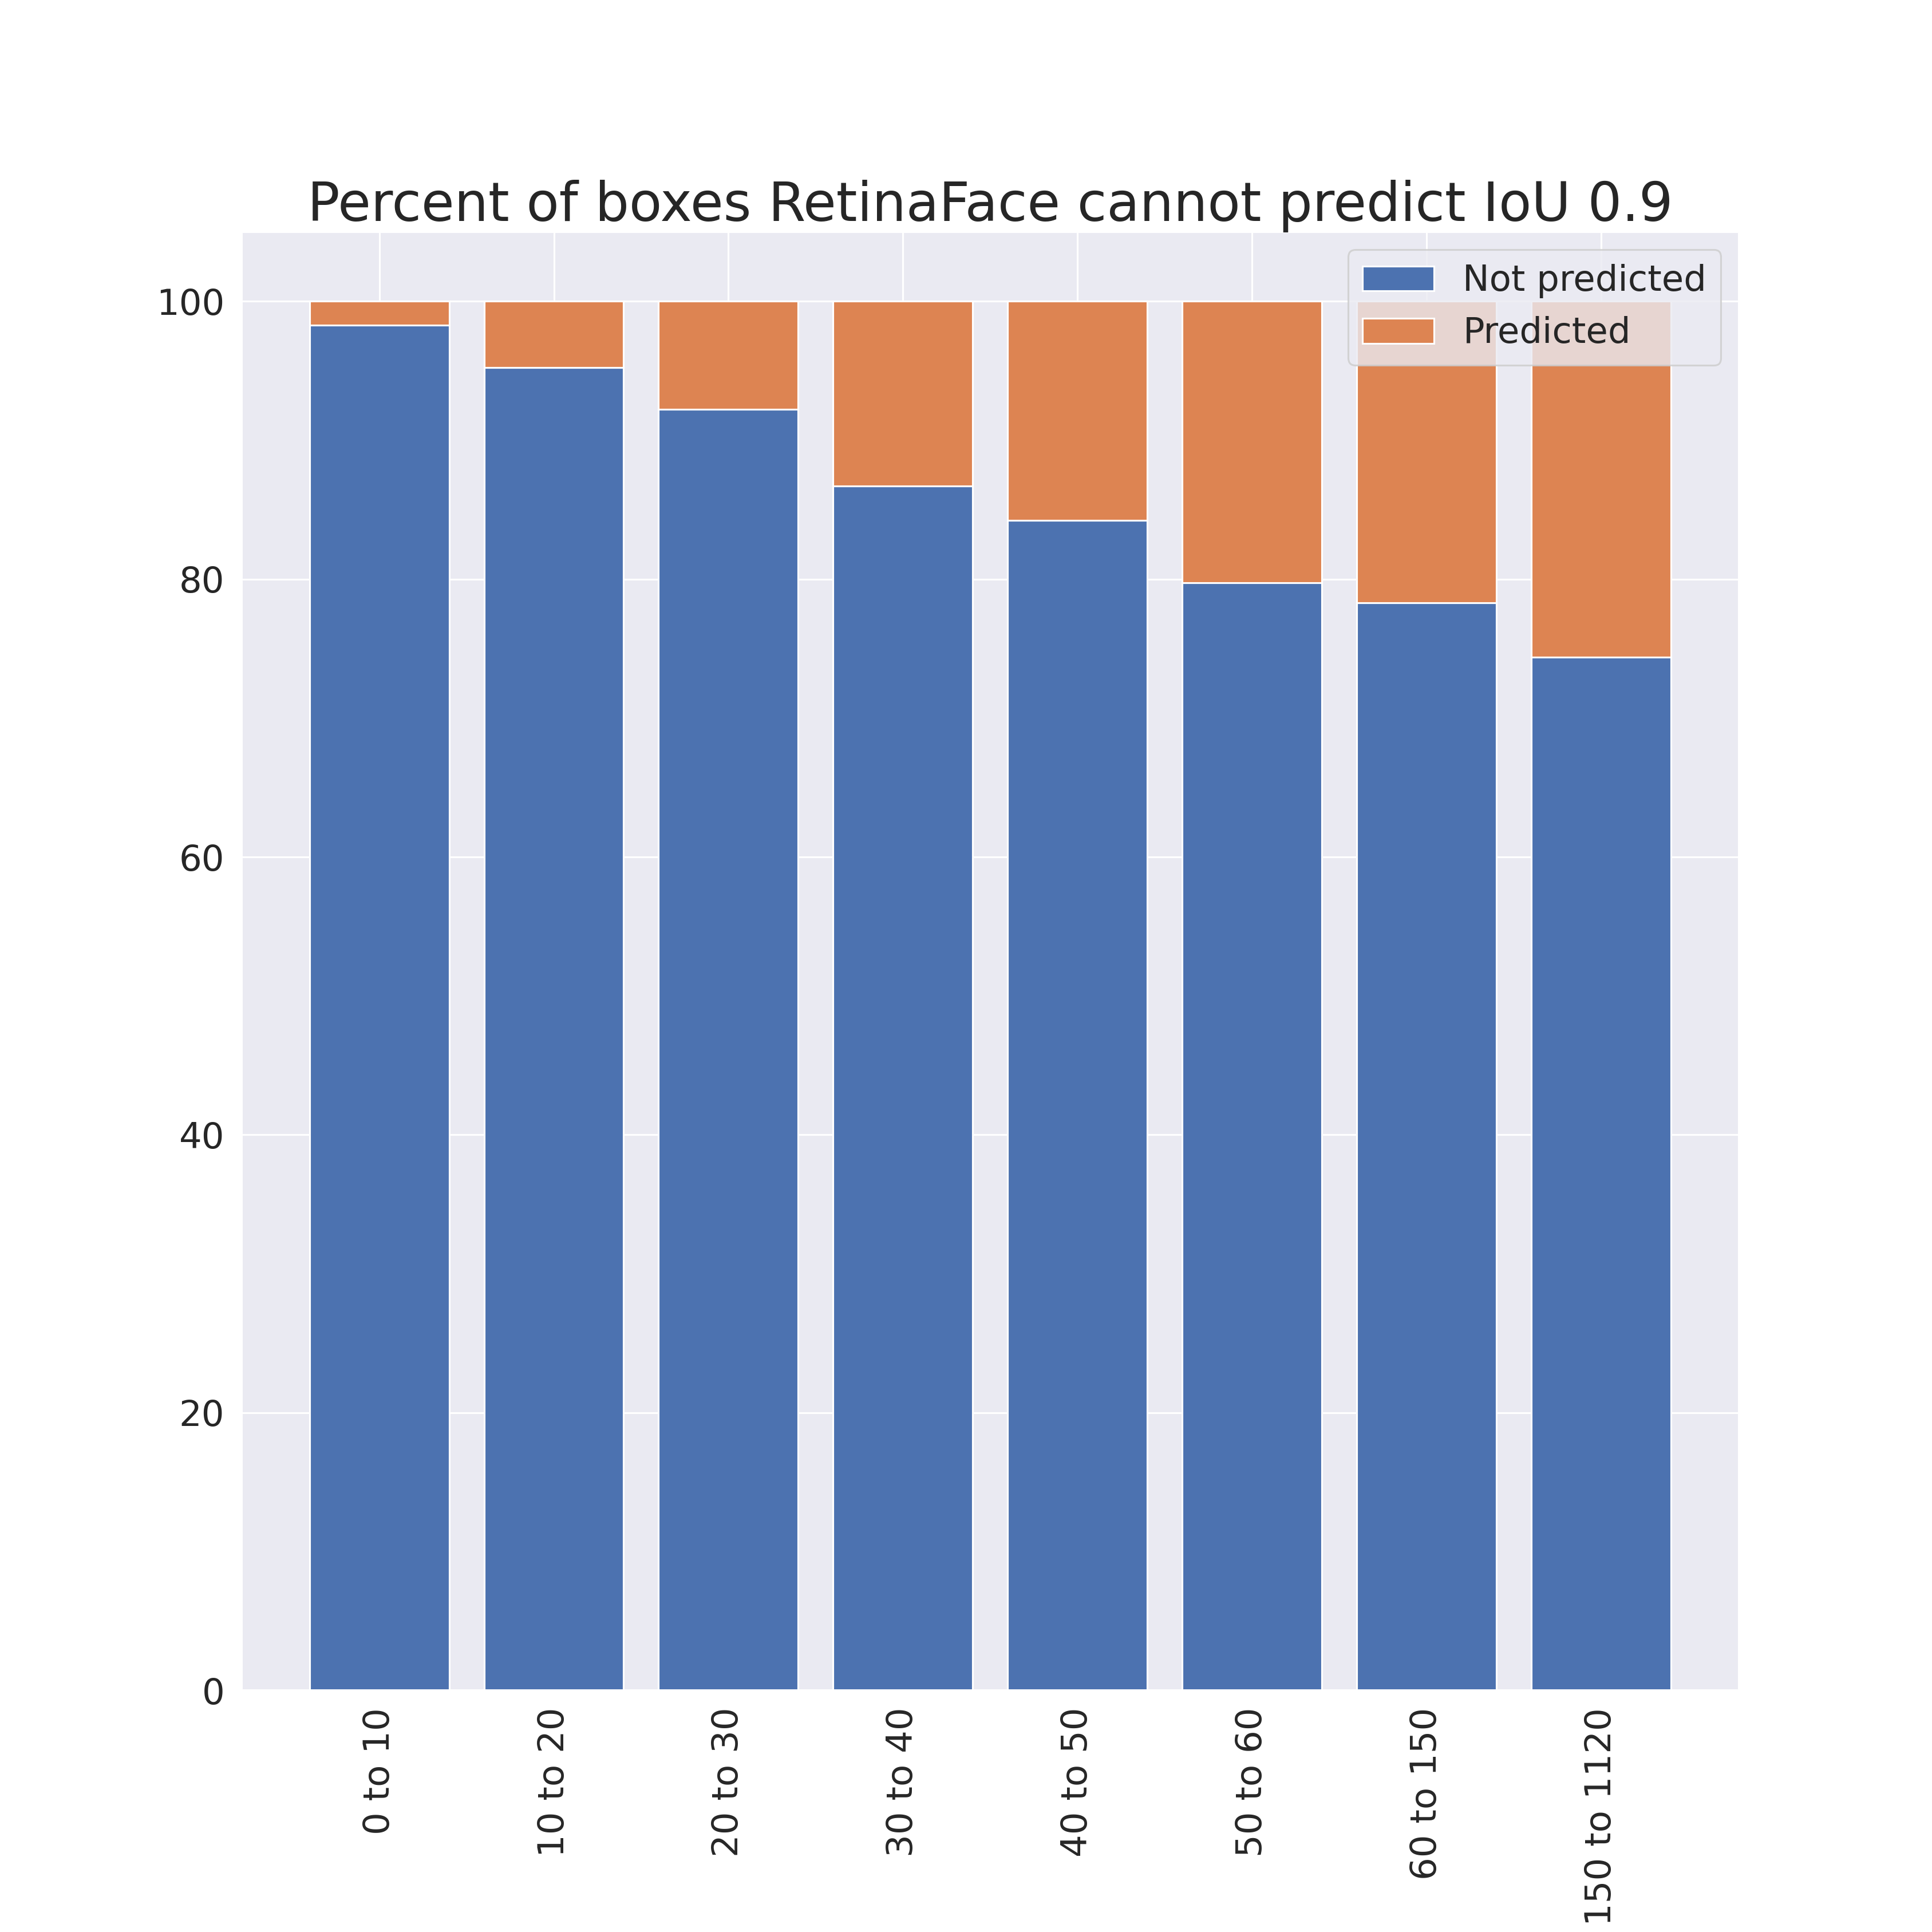
\includegraphics[width=7.3cm, trim={2.5cm 0cm 1.7cm 3.3cm}, clip]{images/retinafocus_iou_90_compare_percent}} 
        \caption{Tỷ lệ số lượng hộp giới hạn\index{hộp giới hạn} mà mô hình RetinaFace dự đoán ra và không dự đoán ra tương ứng với IoU\index{IoU} 0.5 (a), IoU\index{IoU} 0.75 (b), IoU\index{IoU} 0.9 (c)}
        \label{fig:retinafocus_iou_compare_percent}
    \end{figure}

    \noindent
    Tuy nhiên, để nhánh tập trung đối tượng\index{nhánh tập trung đối tượng} hoạt động hiệu quả, ta cần xây dựng được bộ tham số phù hợp với bộ dữ liệu và nhánh xác định đối tượng\index{nhánh xác định đối tượng}.
    Để xây dựng được bộ tham số này, ta cần phân tích điểm yếu của nhánh xác định đối tượng\index{nhánh xác định đối tượng} trên bộ dữ liệu WIDER FACE.
    Từ những điểm yếu, ta lựa chọn bộ tham số của nhánh tập trung đối tượng\index{nhánh tập trung đối tượng} nhằm giúp cho nhánh tập trung đối tượng\index{nhánh tập trung đối tượng} xác định được những vùng mà nhánh xác định đối tượng\index{nhánh xác định đối tượng} dự đoán yếu và zoom in giúp nhánh xác định đối tượng\index{nhánh xác định đối tượng} dự đoán chính xác hơn.
    Trong hình \ref{fig:retinafocus_iou_compare_percent}, trên cả ba mức IoU\index{IoU}, tỷ lệ số lượng hộp giới hạn\index{hộp giới hạn} mà mô hình RetinaFace không dự đoán ra đối với nhóm các hộp giới hạn\index{hộp giới hạn} nhỏ từ 0 điểm ảnh\index{điểm ảnh} đến 30 điểm ảnh\index{điểm ảnh} và đặc biệt là từ 0 điểm ảnh\index{điểm ảnh} đến 10 điểm ảnh\index{điểm ảnh} đều cao vượt trội so với các kích thước hộp giới hạn\index{hộp giới hạn} khác.

    \begin{figure}[H]
        \centering
        \subfigure[]{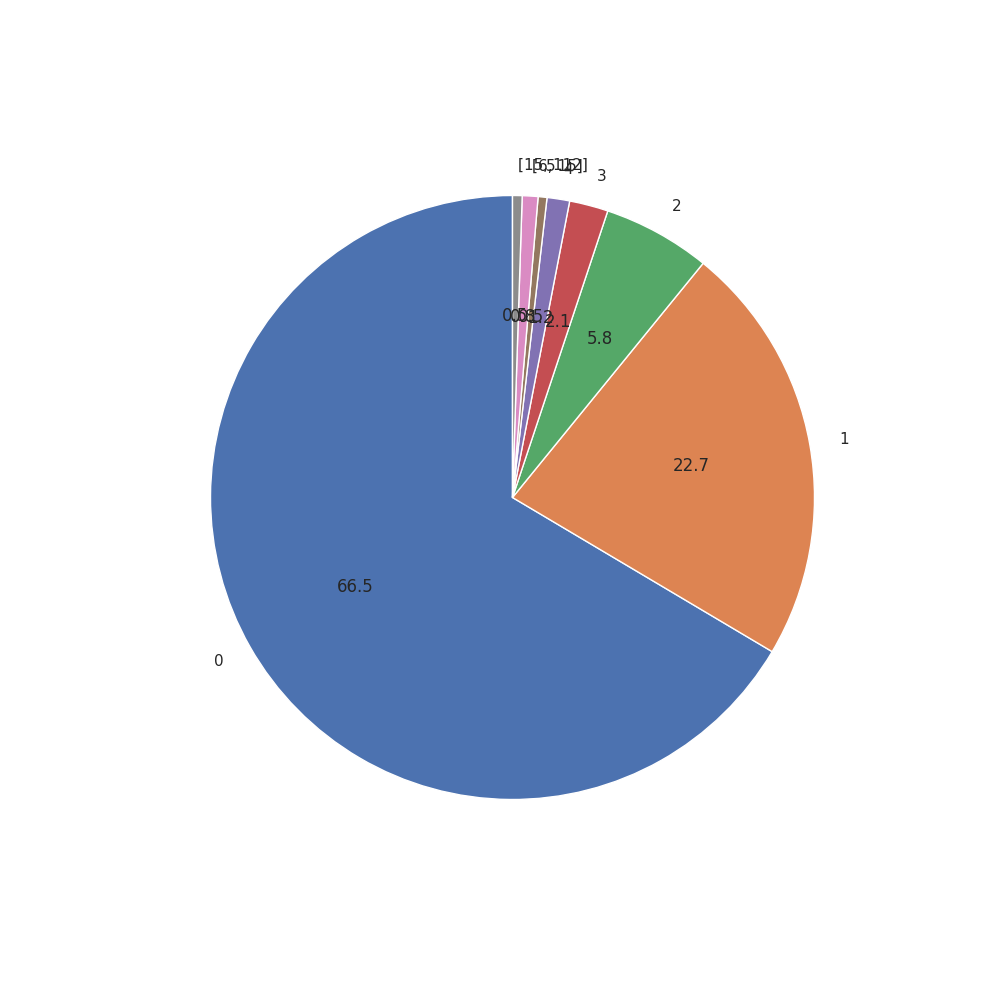
\includegraphics[width=7.3cm, trim={1.1cm 0cm 0.6cm 2cm}, clip]{images/retinafocus_iou_50_lower}} 
        \subfigure[]{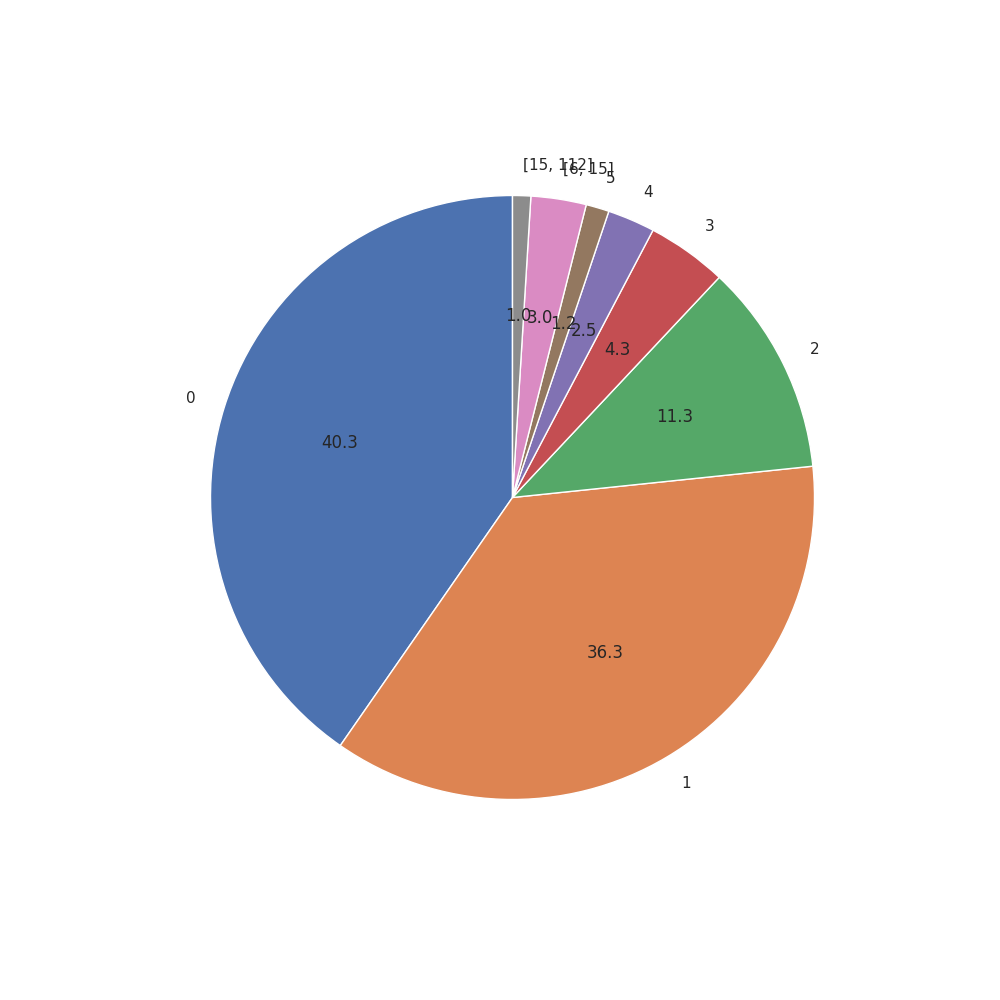
\includegraphics[width=7.3cm, trim={1.1cm 0cm 0.6cm 2cm}, clip]{images/retinafocus_iou_75_lower}} 
        \subfigure[]{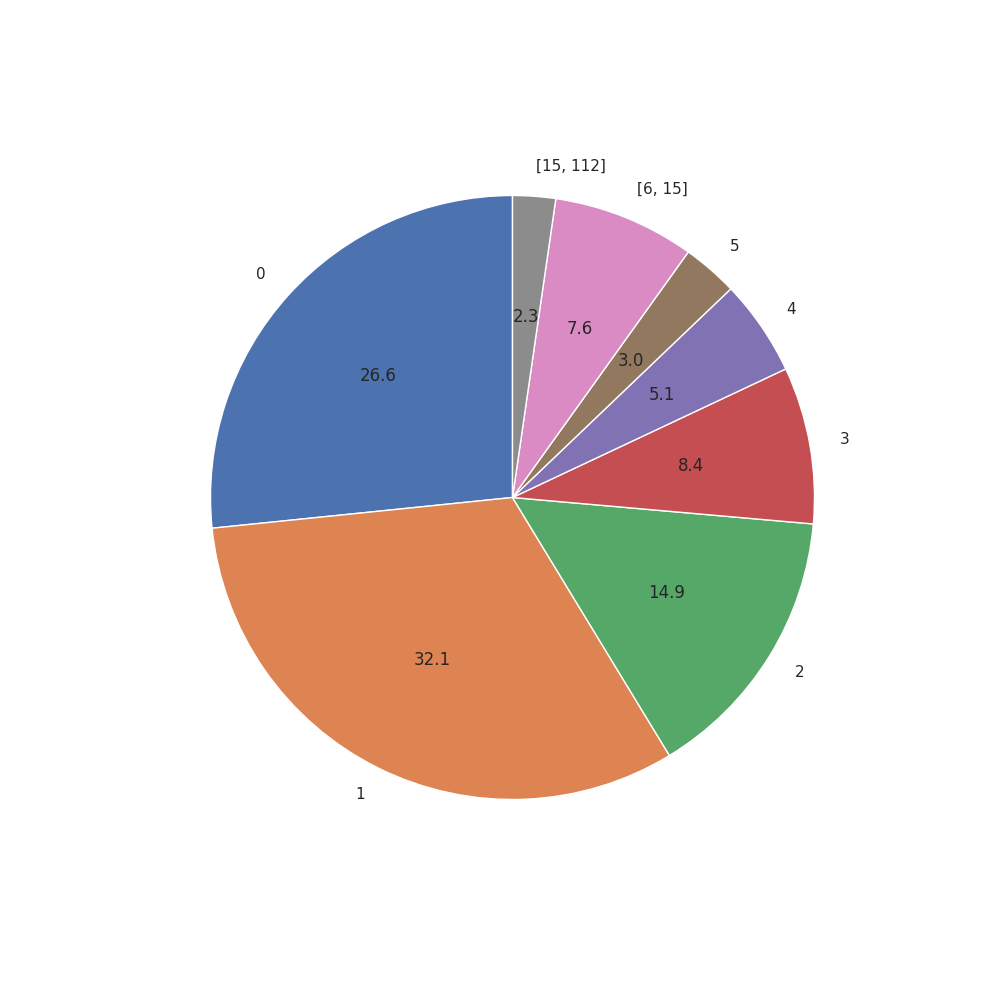
\includegraphics[width=7.3cm, trim={1.1cm 0cm 0.6cm 2cm}, clip]{images/retinafocus_iou_90_lower}} 
        \caption{Tỷ lệ các kích thước của hộp giới hạn\index{hộp giới hạn} mà RetinaFace không dự đoán ra tương ứng với IoU\index{IoU} 0.5 (a), IoU\index{IoU} 0.75 (b), IoU\index{IoU} 0.9 (c)}
        \label{fig:retinafocus_iou_lower}
    \end{figure}

    \noindent
    Cụ thể hơn, trong hình \ref{fig:retinafocus_iou_lower}, dù xét ở mức IoU\index{IoU} nào, thì các hộp giới hạn\index{hộp giới hạn} có kích thước nhỏ từ 0 đến 60 đều chiếm tổng tỷ lệ rất lớn, cụ thể, đối với IoU\index{IoU} 0.5 là 98.7\%, đối với IoU\index{IoU} 0.75 là 96\% và đối với IoU\index{IoU} 0.9 là 90.1\%.

    \noindent
    Hơn nữa, với kiến trúc của FPN như hình \ref{fig:retinafocus_architecture}, một hộp giới hạn\index{hộp giới hạn} có kích thước $4 \times 4$ ở ảnh đầu vào sẽ có tương ứng một khu vực có kích thước $2 \times 2$ ở bản đồ đặc trưng\index{bản đồ đặc trưng} ${C}_{2}$ và ${P}_{2}$, $1 \times 1$ ở bản đồ đặc trưng\index{bản đồ đặc trưng} ${C}_{3}$ và ${P}_{3}$ và gần như không còn thông tin ở các bản đồ đặc trưng\index{bản đồ đặc trưng} từ ${C}_{4}$ và ${P}_{4}$ trở đi.
    Điều này khiến cho các hộp giới hạn\index{hộp giới hạn} này trở thành các điểm dữ liệu nhiễu của nhánh tập trung đối tượng\index{nhánh tập trung đối tượng}, khiến cho việc học của nhánh tập trung đối tượng\index{nhánh tập trung đối tượng} bị giảm hiệu quả.

    \noindent
    Từ những phân tích trên, chúng tôi lựa chọn lần lượt các tham số $a = 5, b = 60, c = 150$ tương ứng với groundtruth\index{groundtruth} hộp giới hạn\index{hộp giới hạn} có kích thước từ $5 \times 5$ đến $60 \times 60$ là các hộp giới hạn\index{hộp giới hạn} cần được focus, các groundtruth\index{groundtruth} hộp giới hạn\index{hộp giới hạn} có kích thước dưới $5 \times 5$ hoặc từ $60 \times 60$ đến $150 \times 150$ là các hộp giới hạn\index{hộp giới hạn} không cần quan tâm và các groundtruth\index{groundtruth} hộp giới hạn\index{hộp giới hạn} có kích thước trên $150 \times 150$ là các hộp giới hạn\index{hộp giới hạn} được coi như là background\index{background}. \\

    \noindent
    \textbf{\textit{Thuật toán sinh Focus Chips}} \\
    Dựa trên AutoFocus \cite{najibi2019autofocus}, sau khi mô hình đã được huấn luyện và dự đoán ra được điểm ảnh\index{điểm ảnh} cần được focus, mô hình cần một thuật toán để crop ra được khu vực cần focus trên ảnh làm đầu vào cho cả hai nhánh xác định đối tượng\index{nhánh xác định đối tượng} và nhánh tập trung đối tượng\index{nhánh tập trung đối tượng} ở nhữnglượt tiếp theo.
    Và đó là vai trò của thuật toán sinh Focus Chips.

    \begin{figure}[H]
        \centering
        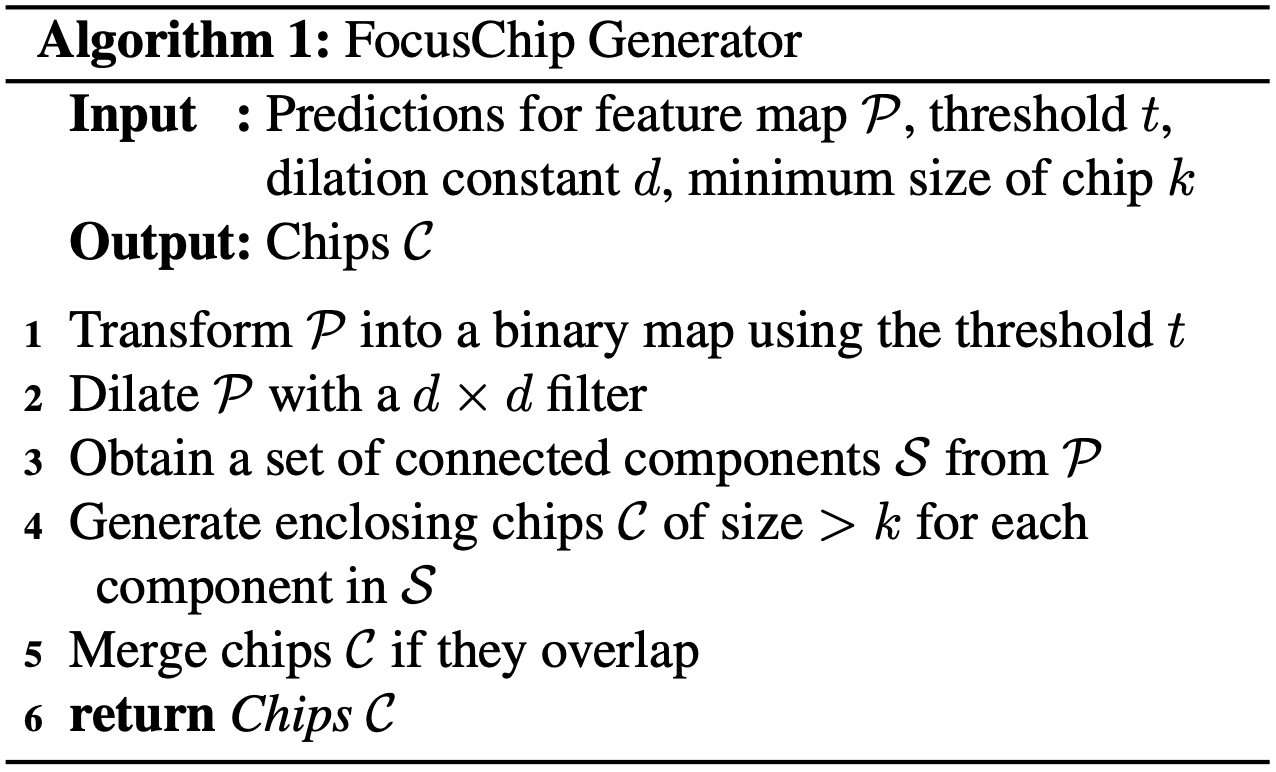
\includegraphics[width=10cm] {images/autofocus_focus_chip_gen}
        \caption{Chi tiết thuật toán sinh Focus Chips (Nguồn: \cite{najibi2019autofocus})}
        \label{fig:autofocus_focus_chip_gen}
    \end{figure}

    \noindent
    Trong quá trình dự đoán, sau khi mô hình đã dự đoán được các điểm ảnh\index{điểm ảnh} cần được focus (ký hiệu là $\mathcal{P}$) trên Focus Pixel  mask, ta biến đổi mask này trở về dạng binary mask bằng threshold $t$.
    Tham số $t$ được sử dụng để cân đối giữa tốc độ và độ chính xác của mô hình (cụ thể với tham số $t$ lớn, số lượng các điểm ảnh\index{điểm ảnh} cần được focus sẽ giảm đi và tốc độ của mô hình AutoFocus sẽ tăng và ngược lại). \\
    Từ binary mask đã được sinh ra ở trên, thuật toán sinh Focus Chips sẽ đưa qua một filter có kích thước $d \times d$ nhằm giãn nở các điểm ảnh\index{điểm ảnh} thêm một chút để thu được các thành phần liên thông $\mathcal{S}$, từ đó có nhiều thông tin hơn khi crop ảnh đầu vào với các focus điểm ảnh\index{điểm ảnh} này. \\
    Cuối cùng, ta crop ra các chip $\mathcal{C}$ với kích thước tối thiểu là $k \times k$ và bao trọn các thành phần liên thông $\mathcal{S}$ trên.
    Các chip trong $\mathcal{C}$ nếu có overlap với nhau sẽ được gộp lại chung thành một chip. \\
    Việc sinh ra các chip $\mathcal{C}$ giúp mô hình AutoFocus có thể sử dụng ý tưởng Image Pyramids nhưng tiết kiệm chi phí tính toán nhờ loại bỏ các khu vực khả năng cao không chứa đối tượng. \\

    \noindent
    \textbf{\textit{Thuật toán Focus Stacking}} \\
    Một vấn đề cần phải giải quyết khi thực hiện dự đoán với ý tưởng Image Pyramids trong bài toán nhận diện đối tượng\index{nhận diện đối tượng} là việc tổng hợp lại các hộp giới hạn\index{hộp giới hạn}.
    Với ý tưởng từ AutoFocus \cite{najibi2019autofocus}, vấn đề này còn phức tạp hơn với trường hợp một đối tượng có kích thước lớn được dự đoán ở kích thước này, nhưng đến kích thước tiếp theo, đối tượng đó bị crop trong quá trình crop chip và trở thành một đối tượng có kích thước nhỏ hơn.
    Nhằm hạn chế bớt vấn đề này, nhóm tác giả chỉ ra rằng \textit{bước 2} trong thuật toán sinh Focus Chips \ref{fig:autofocus_focus_chip_gen} là cực kỳ quan trọng.

    \begin{figure}[H]
        \centering
        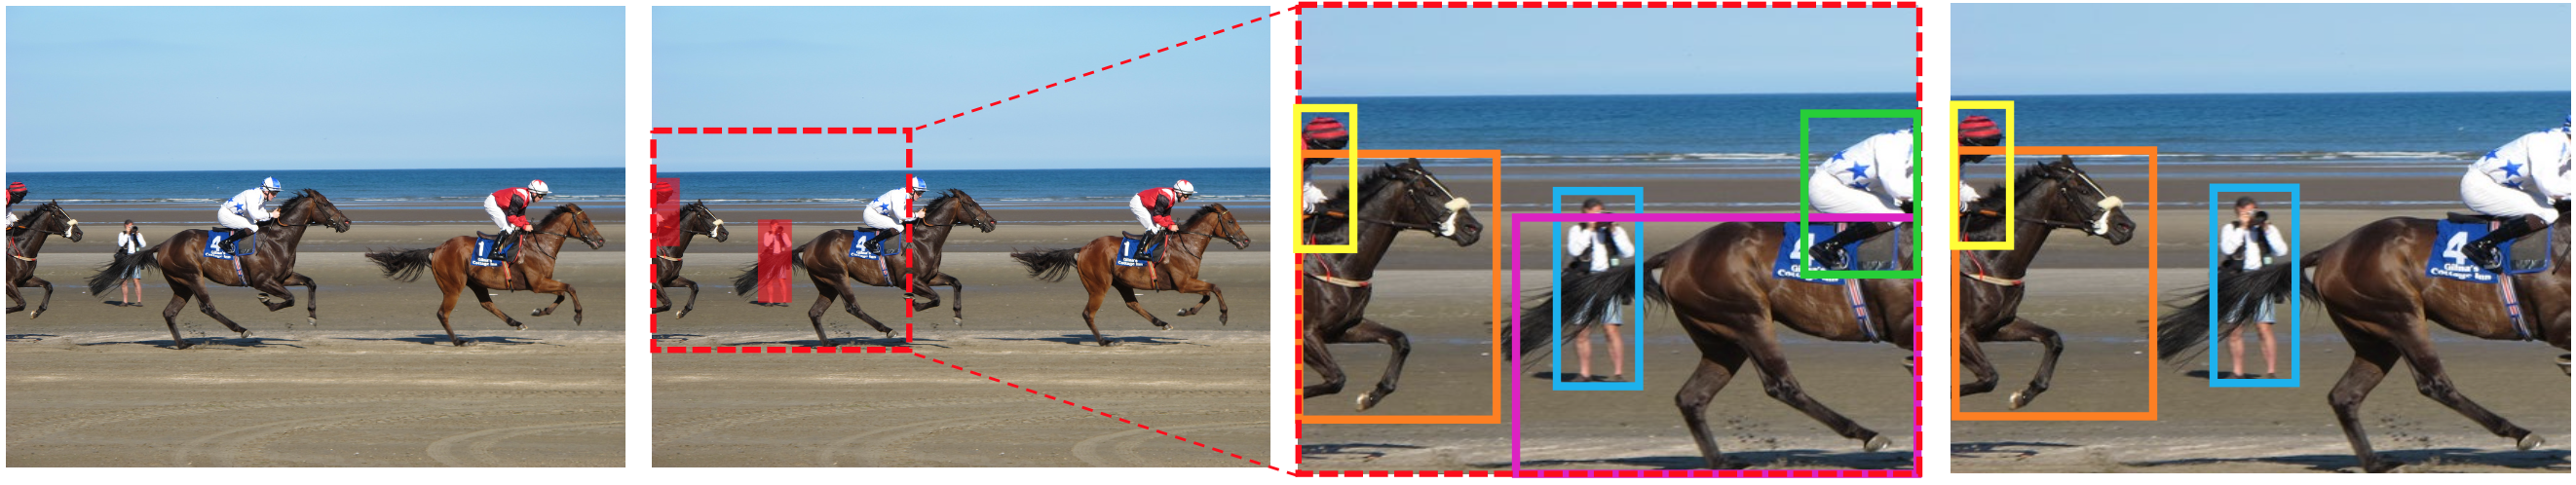
\includegraphics[width=12cm] {images/autofocus_focus_stack}
        \caption{Ví dụ về cơ chế hoạt động của thuật toán Focus Stacking (Nguồn: \cite{najibi2019autofocus})}
        \label{fig:autofocus_focus_stack}
    \end{figure}

    \noindent
    Tuy nhiên, nhóm tác giả cũng đề ra một số luật nhằm loại bỏ các dự đoán lỗi của các đối tượng được định vị trên một focus chip: \\
    - Nếu một đối tượng nằm trên một biên của chip nhưng không phải biên của ảnh đầu vào (nghĩa là đối tượng này đã bị crop sau khi qua thuật toán sinh Focus Chip), thì dự đoán sẽ bị loại bỏ. \\
    - Nếu một đối tượng nằm trên một biên của chip và đó là biên của ảnh đầu vào, nhóm tác giả sẽ tiếp tục kiểm tra biên còn lại của đối tượng, nếu đó là biên của chip, dự đoán sẽ bị loại, còn nếu đó không phải là biên của chip, dự đoán sẽ được giữ lại. \\
    - Nếu một đối tượng nằm trên hai biên của chip và đó đều là hai biên của ảnh đầu vào, nhóm tác giả sẽ giữ lại những dự đoán này. \\
    Sau khi loại bỏ bớt các dự đoán bằng thuật toán Focus Stacking, mô hình AutoFocus đưa ra tổng hợp dự đoán từ các kích thước ảnh khác nhau và là các dự đoán cuối cùng của ảnh đầu vào.
}